\documentclass[utf8, russian, hpadding=5mm, vpadding=15mm, floatsection, columnxxvi, columnxxxi, columnxxxii, equationsection, pointsection, footnoteasterisk]{eskdtext}

\usepackage{ucs}							%хз
\usepackage{cmap}						%решение трабла с крокозябрами в pdf

\usepackage[normalem]{ulem}

\usepackage{setspace}
\usepackage{tocloft}
\usepackage[dvipsnames]{xcolor}
\usepackage{indentfirst}

\usepackage{nameref}
\usepackage{hyperref}
\hypersetup{
    linktoc=all,
    pdftex,
    unicode=true,
    colorlinks=true,
    linkcolor=blue,
    citecolor=red,
    urlcolor=green,
    %linktocpage=true,
    pdfhighlight=/N
}

% подключение дополнительных пакетов
\usepackage{amsfonts, amsmath, amssymb, mathtext}
\newcommand{\No}{\textnumero}

\graphicspath{{./pics/}{./images/}{./pictures/}}
\usepackage{wallpaper}

\renewcommand{\familydefault}{\sfdefault}

\newcommand{\squpp}{\vspace{-4mm}}
\newcommand{\squp}{\vspace{-2mm}}
\newcommand{\sqdownn}{\vspace{2mm}}
\newcommand{\sqdown}{\vspace{1mm}}

\newcommand{\squeezeup}{\vspace{-4mm}}
\newcommand{\squeezeeup}{\vspace{-2mm}}
\newcommand{\squeezeedown}{\vspace{2mm}}
\newcommand{\squeezeeedown}{\vspace{1mm}}

%\renewcommand{\cftaftertoctitle}{\hfill}
\renewcommand{\cfttoctitlefont}{\hspace{7cm}\Large\bfseries}	%KOSTIL'
%\renewcommand{\cftaftertoctitle}{\hfill}
\renewcommand{\cftdot}{.}
\renewcommand{\cftsecleader}{\cftdotfill{\cftdotsep}} % for sections
\makeatletter
\g@addto@macro\cftsecfont{\bfseries}
\g@addto@macro\cftsubsecfont{\bfseries}
\g@addto@macro\cftsubsubsecfont{\bfseries}
\g@addto@macro\cftparafont{\bfseries}
\g@addto@macro\cftsubparafont{\bfseries}
\g@addto@macro\cftsubparafont{\bfseries}
\g@addto@macro\cftfigfont{\bfseries}
\g@addto@macro\cfttabfont{\bfseries}

\g@addto@macro\cftsecpagefont{\bfseries}
\g@addto@macro\cftsubsecpagefont{\bfseries}
\g@addto@macro\cftsubsubsecpagefont{\bfseries}
\g@addto@macro\cftparapagefont{\bfseries} 
\g@addto@macro\cftsubparapagefont{\bfseries}
\g@addto@macro\cftfigpagefont{\bfseries}
\g@addto@macro\cfttabpagefont{\bfseries}
\makeatother


% стиль оформления ссылок на источники
\bibliographystyle{ugost2008}

% Для определения форматирования нумерации элементов списка литературы
\makeatletter
\renewcommand{\@biblabel}[1]{#1}
\makeatother

\ESKDtitle{{\Large Название работы}\\ \small Пояснительная записка}
\ESKDsignature{КСУИ.102.4135.001 ПЗ}
\ESKDgroup{\footnotesize Университет ИТМО\\Кафедра СУиИ\\гр.~R4235}
\ESKDauthor{\resizebox{2.22cm}{\height}{Ватрушкин Н. Ю.}}
%\ESKDchecker{}
%\ESKDnormContr{\resizebox{2.22cm}{\height}{}}
%\ESKDapprovedBy{}

% оступы от заголовков разделов и подразделов
\ESKDsectSkip{section}{7mm}{7mm}
\ESKDsectSkip{subsection}{5mm}{5mm}
\ESKDsectSkip{subsubsection}{3mm}{3mm}


\begin{document}
    \addtocounter{page}{0}
    %\ESKDthisStyle{empty}
\mbox{}
\ThisLRCornerWallPaper{1}{title_page_1.pdf}
\newpage
%\ESKDthisStyle{empty}
%\mbox{}
%\ThisLRCornerWallPaper{1}{title_page2.pdf}
%\newpage

    \ESKDthisStyle{formII}
    \renewcommand{\cftaftertoctitle}{\thispagestyle{empty}}

	\begingroup
		\hypersetup{linkcolor=black}
		\tableofcontents
	\endgroup    
    
    \newpage
    \topmargin = 0 mm
    
    % ---------------------------------    
    	%\cleardoublepage
	\phantomsection
	\addcontentsline{toc}{section}{Введение}
	\section*{Введение}
Текст введения.
\newpage
    \section{Примеры внутреннего <<убранства>>}\label{part_example_of_doc_inside}
\subsection{Оформление доп. объектов}\label{part_pasting_of_extra_objects}
\subsubsection{Вставка рисунков}\label{part_pasting_of_figures}
Пример оформления рисунка~--- см.~ниже по тексту.

\begin{figure}[h]
    \centering
    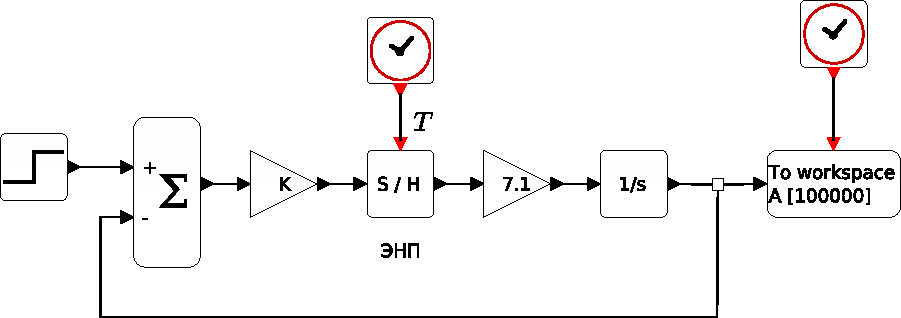
\includegraphics[width=0.7\textwidth]{scheme.pdf}
    \caption{Схема моделирования простенького ОУ.}
    \label{figure_just_example}
\end{figure}


\subsubsection{Вставка таблиц}\label{part_pasting_of_tables}
Пример оформления таблицы~--- см.~ниже по тексту.

\begin{table}[h]
    \caption{Параметры Денавита-Хартенберга.}
    \begin{tabular}{|c|c|c|c|c|}
        \hline
        Звено & $a_i$ & $\alpha_i$ & $d_i$ & $\theta_i$\\
        \hline
        1 & 0 & $\pi/2$ & $l_1$ & $\varphi_1+\pi/2$\\
        \hline
        2  & $l_2$ & $\pi$ & $s_1-2r$ & $\varphi_2-\pi/2$\\
        \hline
        3 & $l_3$ & $-\pi/2$ & $s_2-2r$ & $-\varphi_3$\\
        \hline
        4 & $l_4$ & $-\pi/2$ & $s_3-2r$ & $-\varphi_4$\\
        \hline
        5 & $l_5$ & $-\pi/2$ & $s_4-2r$ & $-\varphi_5$\\
        \hline
        6 & $l_6$ & $-\pi/2$ & $s_5-2r$ & $-\varphi_6$\\
        \hline
    \end{tabular}
    \label{table_DH_params}
\end{table}


\subsubsection{Вставка формул}\label{part_pasting_of_formulas}
Пример оформления формулы:
\begin{equation}\label{eq_example_of_formula}
    W(s) = \cfrac{T_ms+1}{T_ms^2+T_es+1}
\end{equation}
где $T_m$~--- первая постоянная, а $T_e$~--- вторая.


\subsection{Числовые данные ссылок}\label{part_editing_of_refs}
Ссылка на раздел~--- \ref{part_example_of_doc_inside}.
Ссылка на подраздел~--- \ref{part_pasting_of_extra_objects}.
Ссылка на что-то меньшее подраздела~--- \ref{part_pasting_of_figures}.
Cсылка на приложение~--- \ref{append_app_example}.
Ссылка на рисунок~--- \ref{figure_just_example}.
Ссылка на таблицу~--- \ref{table_DH_params}.
Ссылка на формулу~--- \eqref{eq_example_of_formula}.
Ссылка на источник~--- \cite{UrcolaIROS08}\footnote{Описание описания источника~--- см.~used\_books.bib.}.
\newpage
    \section*{Заключение}
\addcontentsline{toc}{section}{Заключение}
Текст заключения
\newpage
    
    \renewcommand\refname{Список использованных источников}
        \begin{thebibliography}{99}
    	%	\addcontentsline{toc}{section}{Список использованных источников}
    	%	\vspace{-1cm}
    	%{\small
    	%\hypertarget{Yang}{}
    	\bibitem{HRI} The Encyclopedia of Human-Computer Interaction / Mads Soegaard, Rikke Friis Dam --- The Interaction Design Foundation, 2nd Ed.
    	
    	\bibitem{Folding} Adrian A. Canutescu, Roland L. Dunbrack, Cyclic coordinate descent: a robotics algorithm for protein loop closure, Protein Science 12 (5) (2003) 963–972.
    	
    	\bibitem{Buss} Buss S. R. Introduction to inverse kinematics with jacobian transpose, pseudoinverse and damped least squares methods //IEEE Journal of Robotics and Automation. – 2004. – Т. 17. – No. 1-19. – С. 16.
    	
    	\bibitem{Balestrino} A. Balestrino, G. De Maria, and L. Sciavicco. Robust control of robotic manipulators. In Proceed-
    	ings of the 9th IFAC World Congress, volume 5, pages 2435–2440, 1984.
    	
    	\bibitem{Wolovich} W. A. Wolovich and H. Elliott. A computational technique for inverse kinematics. The 23rd IEEE
    	Conference on Decision and Control, 23:1359–1363, December 1984.
    	
    	\bibitem{Buss2} Samuel R. Buss and Jin-Su Kim. Selectively damped least squares for inverse kinematics. Journal of Graphics Tools, 10(3):37–49, 2005.
    	
    	\bibitem{Pechev} Alexandre N. Pechev. Inverse kinematics without matrix invertion. In Proceedings of the 2008 IEEE International Conference on Robotics and Automation, pages 2005–2012, Pasadena, CA, USA, May 19-23 2008.
    	
    	
    	\bibitem{Fletcher} R. Fletcher. Practical methods of optimization; (2nd Ed.). Wiley-Interscience, New York, NY, USA, 1987.
    	
    	\bibitem{Kwan} Kwan W. Chin, B. R. von Konsky, and A. Marriott. Closed-form and generalized inverse kinematics solutions for the analysis of human motion. volume 5, pages 1911–1914, 1997.
    	
    	\bibitem{Steven} Steven M. LaValle. Planning Algorithms. Cambridge University Press, New York, NY, USA, 2006.
    	
    	\bibitem{Li} Li-Chun Tommy Wang and Chih Cheng Chen. A combined optimization method for solving the inverse kinematics problems of mechanical manipulators. IEEE Transactions on Robotics and Automation, 7(4):489–499, 1991.
    	
    	\bibitem{Aristidou} Andreas Aristidou and Joan Lasenby. FABRIK: a fast, iterative solver for the inverse kinematics
    	problem. Submitted to Graphical Models, 2010.
    	%}
    	
    \end{thebibliography} 


    \ESKDappendix{обязательное}{Название приложения}\label{append_app_example}
Текст приложения
    
\end{document}